%---------------------------------------------------------------------
%	个性化信息
%--------------------------------------------------------------------
\newcommand{\MYTITLE}{污秽之世,美丽之笼}  %论文标题
\newcommand{\MYID}{2018300000}  %学号
\newcommand{\MYNAME}{藤原妹红}  %姓名
\newcommand{\MYSCHOOL}{金融学院}  %学院
\newcommand{\MYMAJOR}{博丽神社}  %专业
\newcommand{\MYADVISOR}{上白泽慧音}  %指导教师
\newcommand{\MYDATE}{2022年1月7日}  %日期
%---------------------------------------------------------------------
%   各种导言
%--------------------------------------------------------------------
\documentclass[a4paper,12pt]{report}

\usepackage{geometry} % to change the page dimensions
\geometry{a4paper,left=2.5cm,right=2.5cm,top=2.54cm,bottom=2.54cm}%页边距
\usepackage{ctex}
\usepackage{xeCJK}
\usepackage{comment}
\usepackage{setspace}
\usepackage{fancyhdr}
\usepackage{graphicx}
\usepackage{wrapfig}
\usepackage{subfigure}
\usepackage{array}
\usepackage{titlesec}
\usepackage{titletoc}
\usepackage[titletoc]{appendix}
\usepackage{listings}
\usepackage{scrextend}
\usepackage[perpage]{footmisc}
%---------------------------------------------------------------------
%   脚注设置
%--------------------------------------------------------------------
\usepackage{pifont}
\renewcommand\thefootnote{\ding{\numexpr171+\value{footnote}}}
\deffootnote[1em]{1em}{1em}{\zihao{5}\thefootnotemark\space}  %脚注
% 脚注的横线
\renewcommand{\footnoterule}{%
  \kern -3pt
  \hrule width 0.25\paperwidth height 1pt
  \kern 2pt
}
%---------------------------------------------------------------------
%   参考文献设置
%--------------------------------------------------------------------
\usepackage[backend = biber, style = references/gb7714-2015, defernumbers=true]{biblatex}
\renewcommand*{\bibfont}{\small}
\addbibresource{references/bibtest.bib}
\renewcommand{\bibname}{参考文献}
%---------------------------------------------------------------------
%	引用文献设置为上标
%---------------------------------------------------------------------
\begin{comment}
    \makeatletter
    \def\@cite#1#2{\textsuperscript{[{#1\if@tempswa , #2\fi}]}}
    \makeatother
\end{comment}

\lstset{tabsize=4, keepspaces=true,
    xleftmargin=2em,xrightmargin=0em, aboveskip=0.1em,
    %backgroundcolor=\color{gray!20},  % 定义背景颜色
    frame=none,                       % 表示不要边框
    extendedchars=false,              % 解决代码跨页时,章节标题,页眉等汉字不显示的问题
    numberstyle=\ttfamily,
    basicstyle=\ttfamily,
    keywordstyle=\color{blue}\bfseries,
    breakindent=10pt,
    identifierstyle=,                 % nothing happens
    commentstyle=\color{green}\small,  % 注释的设置
    morecomment=[l][\color{green}]{\#},
    numbers=left,stepnumber=1,numberstyle=\scriptsize,
    showstringspaces=false,
    showspaces=false,
    flexiblecolumns=true,
    breaklines=true, breakautoindent=true,breakindent=4em,
    escapeinside={/*@}{@*/},
}
\usepackage{amsmath}
\usepackage{amsthm}
\newtheorem{theorem}{定理}
\newtheorem{definition}{定义}
\newtheorem{corollary}{推论}
\newtheorem{example}{例}
\renewcommand {\thetable} {\arabic{table}}
\renewcommand {\thefigure} {\arabic{figure}}
\usepackage{amsfonts}
\usepackage{lipsum}
%\usepackage{bm}
\usepackage{booktabs} % for much better looking tables
\usepackage{paralist} % very flexible & customisable lists (eg. enumerate/itemize, etc.)
\usepackage{verbatim} % adds environment for commenting out blocks of text & for better verbatim
\usepackage{subfigure} % make it possible to include more than one captioned figure/table in a single float
% These packages are all incorporated in the memoir class to one degree or another...
\usepackage{cases} %equation set
\usepackage{multirow} %use table
\usepackage{algorithm}
\usepackage{algorithmic}
%\usepackage{cite}
\usepackage{hyperref}
\usepackage{longtable}
\usepackage[font={small}]{caption}  % 这样设置表头字体好像是10.95号
\usepackage{zhnumber} % change section number to chinese
\hypersetup{colorlinks,linkcolor=black,anchorcolor=black,citecolor=black, pdfstartview=FitH,bookmarksnumbered=true,bookmarksopen=true,} % set href in tex & pdf
%\usepackage[framed,numbered,autolinebreaks,useliterate]{mcode} % 插入matlab代码
\XeTeXlinebreaklocale "zh"
\XeTeXlinebreakskip = 0pt plus 1pt minus 0.1pt
\setlength{\baselineskip}{22pt}
%---------------------------------------------------------------------
%	图表顺序标号,不分章节
%---------------------------------------------------------------------
\usepackage{chngcntr}
\counterwithout{table}{chapter}
\counterwithout{table}{section}
\counterwithout{figure}{chapter}
\counterwithout{figure}{section}
\counterwithout{equation}{chapter}
\counterwithout{equation}{section}
\titleclass{\chapter}{straight}%禁止chapter换页
%---------------------------------------------------------------------
%	页眉页脚设置
%---------------------------------------------------------------------
\pagestyle{fancy}
\fancyhead[C]{\zihao{5}\MYTITLE}
\lhead{}
\rhead{}
\cfoot{\thepage \\ \textcolor{red}{请注意格式问题可能会导致拒绝答辩。以任何形式采用该模板意味着您已承认:使用该模板而引发的一切负面或正面后果与任何你以外的人都没有任何关系。}}

%---------------------------------------------------------------------
%	调整字体
%---------------------------------------------------------------------
\usepackage[utf8]{inputenc}
\usepackage[OT1]{fontenc}
% \usepackage[T1]{fontenc}
\newcommand{\myfont}{\fontfamily{qtm}\selectfont}
\setCJKmainfont[AutoFakeBold = {2.17}]{宋体}  % 全局中文字体设置
% \setmainfont[AutoFakeBold = {2.17}]{宋体}  %  将全局西文字体也都设置为宋体
\setCJKfamilyfont{songti}[AutoFakeBold = {2.17}]{SimSun}
\setCJKfamilyfont{heiti}[AutoFakeBold = {2.17}]{黑体}
\renewcommand*{\songti}{\CJKfamily{songti}}
% \setmainfont{TeX Gyre Termes}
% \newcommand*{\mysfont}{\fontfamily{timesbd}\selectfont}
%---------------------------------------------------------------------
%	标题格式设置
%---------------------------------------------------------------------
\renewcommand\thesection{(\zhnum{section})}
\renewcommand \thesubsection {\arabic{subsection}.}
\renewcommand \thechapter {\zhnum{chapter}、}
\titleformat{\chapter}{\centering\zihao{4}\songti\bfseries}{\chinese{chapter}、}{0em}{}
\titlespacing{\chapter}{12pt}{12pt}{*3}  %空行直接按照12pt算的,即小四号
\titlespacing{\section}{0pt}{0pt}{*0}
\titlespacing{\subsection}{0pt}{0pt}{*0}
\titleformat{\section}{\zihao{-4}\songti\bfseries}{$\qquad$(\chinese{section})}{0em}{}
\titleformat{\subsection}{\zihao{-4}\songti\mdseries}{$\qquad$\arabic{subsection}.$\ $}{0em}{}
\renewcommand{\figurename}{图}
\renewcommand{\tablename}{表}
%---------------------------------------------------------------------
%	摘要设置
%---------------------------------------------------------------------
%\renewcommand{\abstractname}{摘要}
\newcommand{\enabstractname}{ABSTRACT}
\newcommand{\cnabstractname}{内\quad 容\quad 摘\quad 要}
\newenvironment{enabstract}{%
  \par\small
  \noindent\mbox{}\hfill{{\zihao{3}\selectfont 
  \textbf{\enabstractname}%
  }}\hfill\mbox{}\par
  }{\par}
\newenvironment{cnabstract}{%
  \par\small
  \noindent\mbox{}\hfill{\songti \bfseries \zihao{3} \cnabstractname}\hfill\mbox{}\par
  }{\par}

%---------------------------------------------------------------------
%	目录页设置
%---------------------------------------------------------------------
%\renewcommand{\contentsname}{\zihao{-3} 目\quad 录}
\setcounter{tocdepth}{1}
\renewcommand{\contentsname}{\zihao{3}\bfseries\centering{目$\quad$录}}
\titlecontents{chapter}[0em]{\songti\zihao{4}\bfseries}{\thecontentslabel\ }{}
{\hspace{.5em}\titlerule*[4pt]{$\cdot$}\contentspage}
\titlecontents{section}[2em]{\vspace{0.1\baselineskip}\songti\zihao{4}}{\thecontentslabel\ }{}
{\hspace{.5em}\titlerule*[4pt]{$\cdot$}\contentspage}
%\titlecontents{subsection}[4em]{\vspace{0.1\baselineskip}\songti\zihao{-4}}{\thecontentslabel\ }{}
%{\hspace{.5em}\titlerule*[4pt]{$\cdot$}\contentspage}

%---------------------------------------------------------------------
%	文档开始
%---------------------------------------------------------------------
\begin{document}
\setmainfont[AutoFakeBold = {2.17}]{宋体}
%---------------------------------------------------------------------
%	封面
%---------------------------------------------------------------------
\begin{titlepage}
    \begin{center}
        
\includegraphics[width=0.7\textwidth]{figure/zhongcai.png}\\
        \vspace{8mm}
        \textbf{\zihao{-0}\songti{本科生毕业论文(设计)}}\\\vspace{25mm}
        \textbf{\zihao{2}{\heiti\textbf{\MYTITLE}}}\\[0.8cm]
        \vspace{50mm}
        % \vspace{\fill}
        % \setlength{\extrarowheight}{3mm}
        {\songti\zihao{3}
            \begin{tabular}{rp{8.2cm}<{\centering}}
                % \specialrule{0em}{30pt}
                {\makebox[4\ccwd][s]{学生姓名:}}    & \underline{\makebox[8cm]{\MYNAME}}     \\[10pt]
                {\makebox[4\ccwd][s]{学\qquad 号:}}    & \underline{\makebox[8cm]{\MYID}}       \\[10pt]
                {\makebox[4\ccwd][s]{学\qquad 院:}}    & \underline{\makebox[8cm]{\MYSCHOOL}}     \\[10pt]
                {\makebox[4\ccwd][s]{专\qquad 业:}}    & \underline{\makebox[8cm]{\MYMAJOR}}    \\[10pt]
                {\makebox[4\ccwd][s]{指导教师:}}       & \underline{\makebox[8cm]{\MYADVISOR}}  \\[10pt]
                {\makebox[4\ccwd][s]{日\qquad 期:}}    & \underline{\makebox[8cm]{\MYDATE}}            \\[10pt]
            \end{tabular}
        }\\[2cm]
    \end{center}
\end{titlepage}
%---------------------------------------------------------------------
%  摘要页
%---------------------------------------------------------------------
\setcounter{page}{1}
\thispagestyle{plain}
\begin{cnabstract}
    \vspace{12pt}
    此处是摘要示例,请在abstract.tex中编辑摘要。

    119季秋天,本应是满月的夜晚,月亮却有一点点瑕疵。人类或许难以察觉,但妖怪们却对此十分敏感。
    为了夺回幻想乡的满月,妖怪们各自拉上熟识的人类,博丽灵梦和八云紫、雾雨魔理沙和爱丽丝·玛格特洛依德、十六夜咲夜和蕾米莉亚·斯卡蕾特以及魂魄妖梦和西行寺幽幽子两两一组,停止了夜晚,并踏上了解决异变的道路。
    沿途击败了莉格露·奈特巴格和米斯蒂娅·萝蕾拉后,自机们发现上白泽慧音为了保护人类,用能力将人类村落隐藏了起来。
    战斗过后,自机们在慧音的指引下进入了迷途竹林,并在其中遭遇了同样来调查异变的其他人类主人公。
    战胜对方后,自机们进入永远亭,打败了因幡天为和守护着走廊的铃仙·优昙华院·因幡,最终见到了异变的始作俑者——八意永琳和蓬莱山辉夜。
    从月球逃亡到地上的辉夜,担心满月成为地月之间的通道,进而引来追兵,便命令永琳制造了幻影。虚假之月切断了通道,使地上成为巨大的密室,却也影响了幻想乡中的妖怪。
    辉夜败北后,得知幻想乡有结界保护,月亮上的追兵本就无法到达,便归还了真实之月。
    \par\textbf{关键字:}关键字1 \qquad 关键字2 \qquad 关键字3
\end{cnabstract}
\vspace{12pt}
\setmainfont{Times New Roman}
\begin{enabstract}
    % \begin{myfont}
        \vspace{12pt}
        \lipsum[1]
        \par\textbf{KEY WORDS:} keyword1 \qquad keyword2 \qquad keyword3
    % \end{myfont}
\end{enabstract}
\setmainfont[AutoFakeBold = {2.17}]{宋体}  %  将全局西文字体也都设置为宋体


\newpage

%---------------------------------------------------------------------
%  目录页
%---------------------------------------------------------------------
\thispagestyle{plain}
\setcounter{page}{1}
\begin{spacing}{1.8333} % TODO: 这个行距可能有问题
\tableofcontents % 生成目录
\end{spacing}
\newpage
%---------------------------------------------------------------------
%  引言
%---------------------------------------------------------------------
\begin{center}
    \textbf{\zihao{-3}{\MYTITLE}}
    \\[12pt]
\end{center}
\thispagestyle{plain}
\setcounter{page}{1}

此处为引言示例,请在introduction.tex中编辑引言。

注意页眉从正文开始。

“啊,连续落了两颗呀!”

“嗯。再有一个就十颗了”

两人兴奋的声音在灭了灯的屋内响彻着。差不多快丑时三刻了——连哭泣的孩子都会安静的时刻,然而灵梦和魔理沙两人却没有安静。

店内被两人占据着,并且所有的灯火都被搞灭了。我既不能读书也不能写日记,便借着从窗户洒漏进来的少量月光移动到了两人那里。

“真拿你们两个没办法,已经足够了吧。像这种‘流星群’也不算什么稀奇物……”

“说什么啊。不是香霖说的嘛?今晚的流星群很厉害,一定会落百颗以上啥的”

“我想确实会落百颗以上……难道你打算都看吗?”

“嗯嗯当然了。都准备好一百多个愿望了呢”

——白天的香霖堂店内。

是关于被迫陪着灵梦和魔理沙两人鉴赏流星的日子的事。

我正在凝视着放在桌子上的新入荷的奇妙物品。虽说是新入荷的不过那物品本身却很陈旧,整体都有些脏。用金属制成的部分有着斑斑锈迹。

这个物品,是由稍大一点的西瓜程度的球和用来支撑它的四只脚构成的。球是用金属做的,只是样子非常奇怪。几个像尺子一般细的金属弯曲连接成圈子组合在一起,就好似用竹子做的手鞠,是个空隙很多的球体。并且那些金属圈,还分为能够单个自由回转的和被固定在脚上不能动的两种。

遗憾的是有几个金属圈由于生锈的原因,不能流畅地回转。这个样子的话就不成商品了,所以我在想能否通过自己的手将它再生。

“这满是缝隙的奇怪的地球仪是什么?”

“这不是地球仪哦,魔理沙。还有,你何时进到店里来的?”

“我还以为地球开了一个洞呢”

魔理沙问我,如果不是地球仪的话那究竟是什么?

所谓地球仪,正如其名是地球的模型。幻想乡的住民对自己所居住的星球了解甚少。这是因为幻想乡存在于占据着地球上很少一部分的日本的,极小一部分的深山里,而且还不能从里面走出去。

不过,并不是说外面的情报以及道具就流不进来。地球仪也是从外面世界流入的一个道具,通过它我们就可以了解我们所居住的地球。虽然从知识面来讲已经知道些很细微的事了,但对于幻想乡的人来讲,还不能把自己所居住的大地和知识上的地球联系起来。所以就算说地球开了一个洞,也会很容易就相信了。

然而,看起来像地球仪的这个道具决不是地球仪。是用来测量和地球一样的,平时离幻想乡很近,却又不被详细了解的某种东西的道具。

“这个是名叫‘浑天仪’的道具。地球仪是作为认识地球的道具的话,浑天仪就是用来认识宇宙的道具”

浑天仪,既是一种非常复杂的道具,却又仅仅是测量星星位置的东西而已。

不过它之所以复杂是有原因的。星星看起来好似只是浮着而已,但想要准确测定其位置是很难的。既不能用尺子去量,而且就像远处的地面有山啊森林什么的一样高度也不同。如果夜空也像坐标纸那样引有线,或是有很多作为基准的不动的星星的话就简单了,可那当然是不可能的。观测在双手无法触及的地方的,又没有可以作为基准用的东西的星星的位置这件事,自古以来为难了很多的天文学者。为了解决这个问题,浑天仪便不得不成为一个复杂的道具。
%---------------------------------------------------------------------
%  正文
%---------------------------------------------------------------------
\chapter{子时一刻}
论文引用示例\cite{王宣承-1},按照国标2015格式引用。\footnote{脚注实例,每一页会重新标号}

\section{穢き世の美しき檻}
\begin{table}[h]
    \centering
    \begin{tabular}{lc}
        \toprule[1.5pt]
        成员       & 分工                                        \\
        \midrule[1.0pt]
        博丽灵梦   & 组长、初期报告展示、复制报告汇总            \\
        雾雨魔理沙 & 稳健OLS与FGLS回归估计及分地区、年度差异分析 \\
        东风谷早苗 & 分位数回归、分地区回归、年度差异分析        \\
        十六夜宵夜 & 数据处理、期末汇报展示                      \\
        魂魄妖梦   & 数据处理、中期报告展示、排版整理            \\
        \bottomrule[1.5pt]
    \end{tabular}
\end{table}
\chapter{丑时一刻}
\section{二级标题示例}
\subsection{三级标题示例}
拆行公式:
\begin{equation}
    \begin{split}
        UNEMSEC = \beta_0 + \beta_1HEA\_0 + \beta_2HEA\_1 + \beta_3OLD\_0 +  \\
        \beta_4OLD\_1 + \beta_5ifiwork + \beta_6family\_income + \epsilon
    \end{split}
\end{equation}

\lipsum[1]

\section{玛格特罗伊德}
脚注示例\footnote{って、こりゃまた随分集まったわね。}

「穢き所に、いかでか久しくおはせん。」

そういうと閉ざされた扉は一枚残らず開き――

引用实例,注意该格式未在文件中规定:
\begin{quotation}

永琳、私の力でもう一度だけチャンスをあげる。

これで負けたらその時は……。

そこの人妖!

私の力で作られた薬と永琳の本当の力、
一生忘れないものになるよ!
\end{quotation}

私は輝夜。

\section{线性回归计算peincome、unincome}
\subsection{被解释变量的选择}
关于这两个变量,原文的描述是:
\lipsum[2]

北风卷第白草折,

胡天八月即飞雪

交叉引用示例:表\ref{hhh}
\[
    Ave\_income = \beta_0 + \beta_{1}Ave\_age + \beta_{2}Ave\_edu + \beta_{3}hgender + \beta_{4}hccp + \beta_{5}worker\_ratio + \epsilon
\]


\subsection{解释变量的选择}
これで永夜の術は破れて、夜は明ける!
\begin{table}
    
    \zihao{5}
    \caption{手动插入表格示例}
    \centering
    \begin{tabular}{lcccc}
        \toprule[1.5pt]
        variable & mean & sd   & min   & max   \\
        \midrule[1.0pt]
        SR1      & 0.60 & 0.52 & -5.00 & 1.00  \\
        SR2      & 0.47 & 0.63 & -5.38 & 1.00  \\
        peincome & 9.72 & 0.60 & 7.86  & 11.92 \\
        unincome & 0.00 & 0.74 & -3.35 & 3.71  \\
        PENSION  & 0.78 & 0.42 & 0.00  & 1.00  \\
        HEASEC   & 0.93 & 0.26 & 0.00  & 1.00  \\
        UNEMSEC  & 0.45 & 0.50 & 0.00  & 1.00  \\
        r        & 0.61 & 0.27 & 0.00  & 1.00  \\
        pension  & 0.47 & 0.34 & 0.00  & 1.00  \\
        heasec   & 0.57 & 0.30 & 0.00  & 1.00  \\
        unemsec  & 0.29 & 0.35 & 0.00  & 1.00  \\
        \bottomrule[1.5pt]
    \end{tabular}
    \label{hhh}
\end{table}


\chapter{寅时一刻}
\section{曾依藉的绿}
\begin{figure}[H]
    \centering
    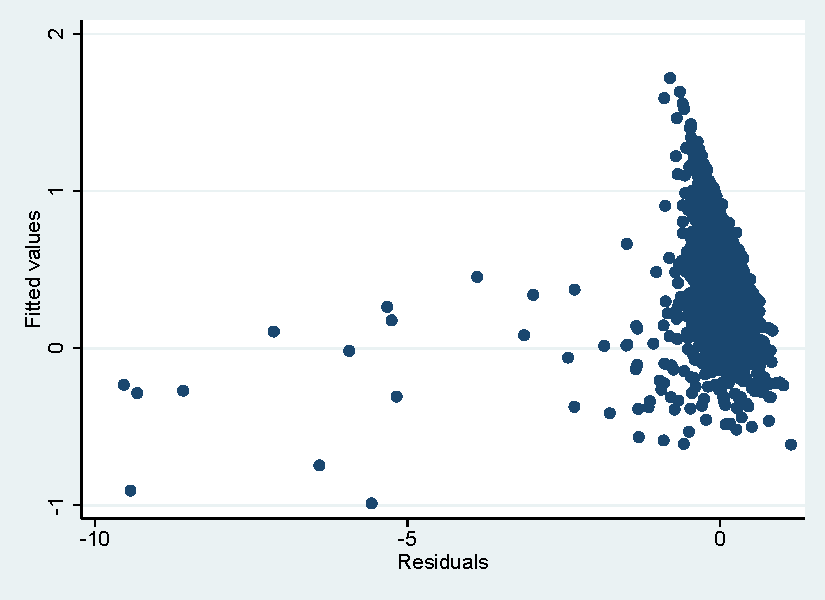
\includegraphics[width=0.65\textwidth]{figure/cancha.pdf}
    \caption{插入图片示例}
\end{figure}


插入代码示例:
\begin{lstlisting}[language=C]
    qui reg SR1 $xx dummy1-dummy24 if time==0
    predict e1,res
    g e2 = e1^2
    g lne2 = log(e2)
    qui reg lne2 peincome if time==0,noc
    predict lne2f
    g e2f =exp(lne2f)
    reg SR1 $xx dummy1-dummy24 if time==0 [aw=1/e2f]
\end{lstlisting}

%---------------------------------------------------------------------
%  其他
%---------------------------------------------------------------------
\vspace{12pt}
\printbibliography
\addcontentsline{toc}{chapter}{参考文献}
\newpage
\chapter*{中央财经大学本科毕业论文(设计)原创性声明}
\addcontentsline{toc}{chapter}{中央财经大学本科毕业论文(设计)原创性声明}
\vspace{1mm}
本人郑重声明:所提交的毕业论文(设计)《\MYTITLE》,
是本人在指导老师的指导下独立进行研究工作所取得的成果。
除文中已经注明引用的内容外,不含任何其他个人或集体已经发表或撰写过的作品成果,
不存在购买、由他人代写、剽窃和伪造数据等作假行为。
对本文研究/设计做出重要贡献的个人和集体,均已在文中以明确方式标明。
本人完全意识到本声明的法律结果,如违反有关规定或上述声明,愿意承担由此产生的一切后果。
\\[50pt]
作者签名:\hfill 年 \quad 月 \quad 日\\
\newpage
\chapter*{致谢}
\addcontentsline{toc}{chapter}{致谢}
それはともかく、そんなぬるいゲームの二次創作はどうかというと、こ
れがまた熱い(笑)。先に言ったとおりこのゲームの特徴は、弾幕がキャ
ラクターとストーリーを語る所。この部分を意識しているのかしていない
のか判りませんが、頂いたどの作品もちゃんとキャラクターが強くて楽し
まさせていただきました。キャラクターの強さは弾幕の強烈さと同義です。
(頂いた作品は全て見させて頂いた後、全て保管してあります。既に数百
作品にものぼるという。)個々の作品に対しての感想は私の立場上、公の
場で余り言う事が出来なくなってしまいましたが、それは個々に挨拶する
時に……。
\newpage
\chapter*{附录}
\addcontentsline{toc}{chapter}{附录}
插入代码示例:
\begin{lstlisting}[language=C]
    qui reg SR1 $xx dummy1-dummy24 if time==0
    predict e1,res
    g e2 = e1^2
    g lne2 = log(e2)
    qui reg lne2 peincome if time==0,noc
    predict lne2f
    g e2f =exp(lne2f)
    reg SR1 $xx dummy1-dummy24 if time==0 [aw=1/e2f]
\end{lstlisting}

\end{document}
